% =============================================================================
\section*{Compl\'ement : Vitesse relative}
\addcontentsline{toc}{section}{Compl\'ement : Vitesse relative}
% =============================================================================

En navigation, il est souvent n\'ecessaire de tenir compte du \textbf{courant} ou du \textbf{vent} pour d\'eterminer la vitesse r\'eelle d'un navire par rapport au fond marin ou \`a un point fixe.

\begin{definition}[title=Vitesse relative]
La \textbf{vitesse relative} d'un objet A par rapport \`a un objet B est la vitesse de A telle que la percevrait un observateur situ\'e sur B :
\begin{equation}
\vec{v}_{A/B} = \vec{v}_A - \vec{v}_B
\end{equation}
\end{definition}

\begin{remarque}[title=Terminologie maritime]
\begin{itemize}
    \item \textbf{Vitesse surface} ($\vec{v}_{surface}$) : vitesse du navire par rapport \`a l'eau (mesur\'ee par le loch)
    \item \textbf{Vitesse fond} ($\vec{v}_{fond}$) : vitesse du navire par rapport au fond marin (mesur\'ee par GPS)
    \item \textbf{Courant} ($\vec{v}_{courant}$) : vitesse de l'eau par rapport au fond
\end{itemize}

La relation fondamentale est :
\begin{equation}
\vec{v}_{fond} = \vec{v}_{surface} + \vec{v}_{courant}
\end{equation}
\end{remarque}

\begin{exemple}{Navire contre le courant}{navire-contre-courant}
Un cargo navigue vers l'est \`a $\SI{12}{n\oe{}uds}$ (vitesse surface). Le courant porte vers l'ouest \`a $\SI{3}{n\oe{}uds}$.

Quelle est la vitesse fond du cargo?

\textbf{Solution :}

En prenant l'est comme direction positive :
\begin{itemize}
    \item $v_{surface} = +\SI{12}{n\oe{}uds}$ (vers l'est)
    \item $v_{courant} = -\SI{3}{n\oe{}uds}$ (vers l'ouest)
\end{itemize}

\[ v_{fond} = v_{surface} + v_{courant} = 12 + (-3) = \SI{9}{n\oe{}uds} \text{ vers l'est} \]

Le navire avance effectivement \`a $\SI{9}{n\oe{}uds}$ par rapport au fond.
\end{exemple}

\begin{exemple}{Travers\'ee avec courant lat\'eral --- Décomposition vectorielle}{traversee-courant-lateral}
Un traversier doit rejoindre un quai situ\'e exactement au nord, \`a $\SI{2}{km}$. Sa vitesse propre (surface) est de $\SI{10}{n\oe{}uds}$, mais un courant de $\SI{3}{n\oe{}uds}$ porte vers l'est.

\textbf{Problème :} Si le capitaine pointe directement vers le nord, le navire dérivera vers l'est. Pour atteindre le quai, il doit \textbf{compenser} en pointant légèrement vers l'ouest.

\begin{center}
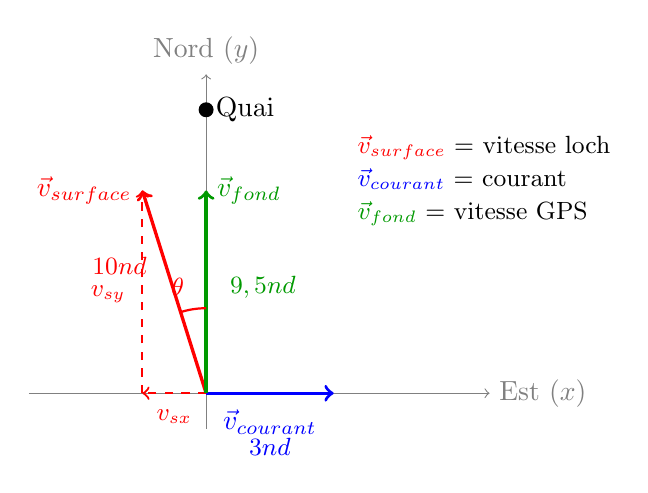
\begin{tikzpicture}[scale=0.9]
% Axes
\draw[gray, ->] (-2.5,0) -- (4,0) node[right] {Est ($x$)};
\draw[gray, ->] (0,-0.5) -- (0,4.5) node[above] {Nord ($y$)};
% Courant (horizontal vers l'est)
\draw[very thick, blue, ->] (0,0) -- (1.8,0);
\node[blue, below] at (0.9,-0.1) {$\vec{v}_{courant}$};
\node[blue, below] at (0.9,-0.5) {\small $\SI{3}{nd}$};
% Vitesse surface (inclinée pour compenser) - angle θ ouest du nord
% sin(17.46$^\circ$) = 0.3, cos(17.46$^\circ$) = 0.954
\draw[very thick, red, ->] (0,0) -- ({-3*sin(17.46)},{3*cos(17.46)}) node[left] {$\vec{v}_{surface}$};
\node[red, left] at (-0.7,1.8) {\small $\SI{10}{nd}$};
% Composantes de la vitesse surface (en pointillés)
\draw[red, dashed, thick, ->] (0,0) -- ({-3*sin(17.46)},0);
\node[red, below] at ({-0.5*3*sin(17.46)},-0.1) {\small $v_{sx}$};
\draw[red, dashed, thick, ->] ({-3*sin(17.46)},0) -- ({-3*sin(17.46)},{3*cos(17.46)});
\node[red, left] at ({-3*sin(17.46)-0.1},1.4) {\small $v_{sy}$};
% Vitesse fond (résultante vers le nord)
\draw[very thick, green!60!black, ->] (0,0) -- (0,{3*cos(17.46)}) node[right] {$\vec{v}_{fond}$};
\node[green!60!black, right] at (0.2,1.5) {\small $\SI{9,5}{nd}$};
% Angle
\draw[thick, red] (0,1.2) arc (90:107.46:1.2);
\node[red] at (-0.4,1.5) {\small $\theta$};
% Point d'arrivée
\fill (0,4) circle (3pt) node[right] {Quai};
% Légende
\node[align=left, anchor=west] at (2,3) {\small \textcolor{red}{$\vec{v}_{surface}$} = vitesse loch\\
\small \textcolor{blue}{$\vec{v}_{courant}$} = courant\\
\small \textcolor{green!60!black}{$\vec{v}_{fond}$} = vitesse GPS};
\end{tikzpicture}
\end{center}

\textbf{Analyse par décomposition vectorielle :}

Pour que $\vec{v}_{fond}$ soit dirigée exactement vers le nord, sa composante $x$ doit être nulle :
\begin{align*}
v_{fond,x} &= v_{surface,x} + v_{courant,x} = 0 \\
-v_{surface}\sin\theta + v_{courant} &= 0
\end{align*}

D'où l'\textbf{angle de compensation} :
\[ \sin\theta = \frac{v_{courant}}{v_{surface}} = \frac{3}{10} = 0{,}3 \quad \Rightarrow \quad \boxed{\theta = 17{,}5^\circ \text{ ouest du nord}} \]

\textbf{Vitesse fond r\'esultante} (composante $y$) :
\[ v_{fond} = v_{fond,y} = v_{surface}\cos\theta = 10 \times \cos(17{,}5^\circ) = \boxed{\SI{9{,}5}{n\oe{}uds}} \]

\textbf{Vérification} par le théorème de Pythagore :
\[ v_{surface}^2 = v_{fond}^2 + v_{courant}^2 \quad \Rightarrow \quad 10^2 = 9{,}5^2 + 3^2 = 90{,}25 + 9 = 99{,}25 \approx 100 \quad \checkmark \]
\end{exemple}

\begin{attention}
La vitesse relative est un concept vectoriel. En 2D, il faut d\'ecomposer les vitesses en composantes et les additionner vectoriellement. Ce sujet sera approfondi dans le cours de navigation.
\end{attention}